\documentclass{beamer}
\usetheme{Pittsburgh}
\beamertemplatenavigationsymbolsempty


\usepackage{amsmath}
\usepackage{amssymb}
\usepackage{graphicx}


\usepackage{subfigure}
\usepackage{multirow}
\usepackage{multicol}
\usepackage{color}
\usepackage{url}
\usepackage{hyperref}
\usepackage{listings}
\usepackage{algorithm}
\usepackage{physics}
% add image path
\graphicspath{{../Images/}}

\title{Accelerating Numerical Simulations using Data-Driven Correction}
\author{Andrea Bonifacio}

\begin{document}

\begin{frame}
\titlepage
\end{frame}


\begin{frame}{Introduction}

    \textbf{Why This Matters}
    \begin{itemize}
        \item \textbf{Challenge}: High-fidelity numerical simulations are computationally expensive, limiting their use in real-time and large-scale scenarios.
        \item \textbf{Trade-off}: Higher accuracy $\rightarrow$ Increased computational cost.
    \end{itemize}
    
    \vspace{0.5cm}
    
    \textbf{Our Idea}
    \begin{itemize}
        \item Integrate insights from accurate simulations into less accurate ones to achieve:
        \begin{itemize}
            \item Comparable accuracy.
            \item Drastically reduced computational time.
        \end{itemize}
    \end{itemize}
    
    \vspace{0.5cm}
    
    \begin{itemize}
        \item \textbf{Generalizable}: Independent of geometry and topology.
        \item \textbf{Transparent}: Avoids black-box methodologies.
        \item \textbf{Efficient}: Prioritizes speed and computational feasibility.
    \end{itemize}
    
    \vspace{0.5cm}
    
    \end{frame}

\begin{frame}
\frametitle{Goal}
\begin{columns}
    \column{0.5\textwidth}
    The \textbf{ideal} method should be:
    \begin{itemize}
    \item Geometry-independent.
    \item Topology-independent.
    \item Not a black-box.
    \item Fast.
    \end{itemize}
    \column{0.5\textwidth}
    The proposed method is:
    \begin{itemize}
    \item[] X
    \item[] \checkmark
    \item[] \checkmark
    \item[] \checkmark
    \end{itemize}
\end{columns}
\end{frame}

\begin{frame}
\frametitle{Similar Works}
Even though we are not aware of any work that uses the same methodology in the field of computational mechanics, there are some works that are related to ours:
\begin{itemize}
    \item \href{https://www.sciencedirect.com/science/article/abs/pii/S0045793023001962}{Data-driven correction of coarse CFD grids}: This is the \textbf{most similar work} to ours and also the inspiration for our work. The authors use various ML techniques to correct the solution obtained on a coarse mesh.
    \item \href{https://arxiv.org/pdf/2109.09491}{A physics-aware framework for real time simulation}: While the approach is different, the \textbf{goal is similar} to ours and can be used as a \textbf{reference}.
    \item \href{https://arxiv.org/abs/1904.06197}{Simulation of hyperelastic materials in real-time using Deep Learning}: This is a similar work to the previous one, in which the author uses a neural network to \textbf{predict the deformation} of a hyperelastic material. Due to missing implementation in our numerical solver, we stick to \textbf{linear elasticity}.
\end{itemize}
\end{frame}






\begin{frame}
\frametitle{Methodology}
Consider a general boundary value problem:
\[
    \begin{split}
        \text{Find } u \text{ such that } \mathcal{L}u = f \text{ in } \Omega,\\
        B.C. \text{ on } \partial \Omega,
    \end{split}
\]
where \(\mathcal{L}\) is a differential operator, \(f\) is a source term, \(\Omega\) is the domain and \(\partial \Omega\) is the boundary of the domain. 

\vspace{0.5cm}
To solve it numerically, the domain is discretized into two meshes: a coarse mesh and a fine mesh and the force is applied on a subdivision of the boundary made to avoid applying the force too close to the Dirichlet boundary conditions. 
\end{frame}

\begin{frame}
\frametitle{Methodology}
\begin{itemize}
    \item The domain \( \Omega \) is discretized into two meshes \( \Omega_c \) and \( \Omega_f \) with \( n_c \) and \( n_f \) nodes respectively. 
    \item The solution associated with the fine mesh is denoted by \( u^f \) and the solution associated with the coarse mesh is denoted by \( u^c \).
    \item A set of points \(G \subset \Omega\) is chosen as a mutual grid for the two meshes.
    \item The solutions are interpolated on the mutual grid: \( u^f \approx u^f_G \) and \( u^c \approx u^c_G \).
    \item Now that both solutions live in the same space, the difference between them can be computed: \( e = u^f_G - u^c_G \).
\end{itemize}
\end{frame}

\begin{frame}
\frametitle{Methodology}
\begin{itemize}
    \item A dataset \(\mathcal{D} = \{{u_G^c}_i, e_i\}_{i=1}^N\) is created by solving the problem on \(N\) different random simulations.
    \item A neural network is trained on the dataset.
    \item On a new simulation, the coarse solution is computed and its correction is obtained as: 
    \[
        \tilde{u}_G^c = u_G^c + \mathcal{NN}(u_G^c).
    \]
    \item Using RBF interpolation, the corrected solution is reconstructed on the mesh \( \Omega_c \):
    \[
        \tilde{u}^c = \text{RBF}(\tilde{u}_G^c).
    \]
\end{itemize}
\end{frame}

\begin{frame}
\frametitle{Boundary Conditions}
Even though the information about the boundary conditions could be already included in the solution, we tried to enforce them explicitly.
\begin{itemize}
    \item Given the vector of the solution \( u_G^c \), we take the vector of the boundary conditions \( b \) and concatenate them.
    \item The vector \( b \) contains the direction of the force, its magnitude and the boundaries of the box where the force is applied.
    \item In the case of a graph dataset, the boundary conditions are included in the node features.
    \end{itemize}

\end{frame}


\begin{frame}
\frametitle{Pros and Cons}
\begin{columns}
    \column{0.5\textwidth}
    Pros:
    \begin{itemize}
        \item Avoid the black-box approach of other methods.
        \item Once trained on a single coarse mesh, the model works well even for different topologies.
        \item The small size of the model allows for fast computations.
    \end{itemize}
    \column{0.5\textwidth}
    Cons:
    \begin{itemize}
        \item This method is still geometry dependent.
        \item Need a large dataset to train the model (for now).
    \end{itemize}
\end{columns}
\end{frame}

\begin{frame}
    \frametitle{Numerical Results}
    To test the method, two different linear elasticity problems were solved:
    \begin{itemize}
        \item A 2D beam
        \item A 3D beam
    \end{itemize}
    \begin{columns}
        \column{0.5\textwidth}
        \begin{figure}
            \centering
            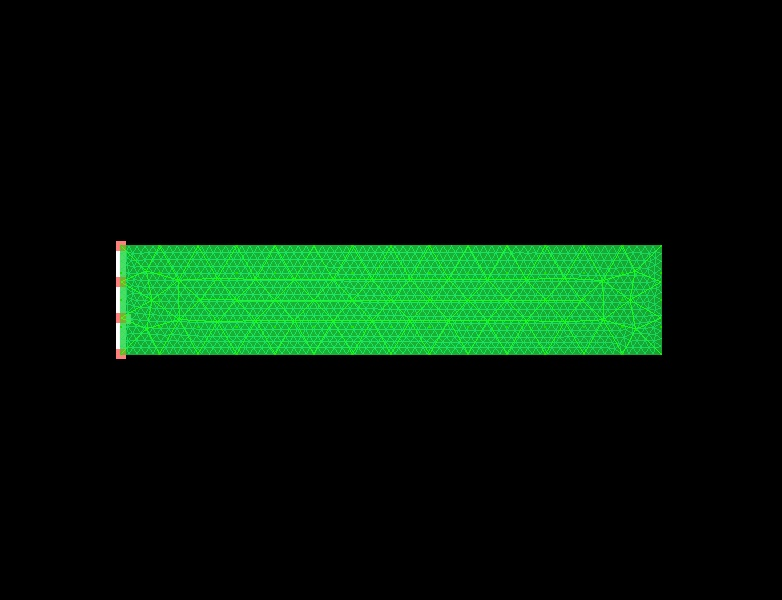
\includegraphics[width=0.8\textwidth]{Images/2D_beam.png}
            \caption{2D Beam}
        \end{figure}
        \column{0.5\textwidth}
        \begin{figure}
            \centering
            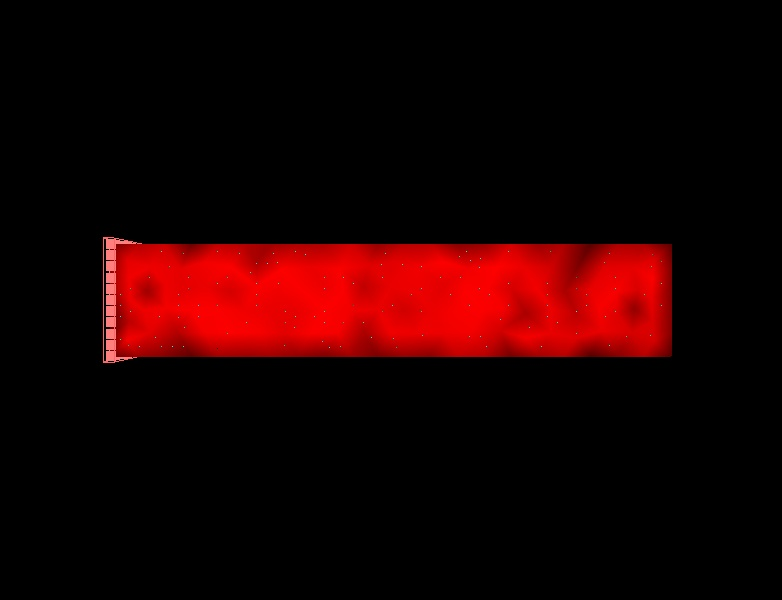
\includegraphics[width=0.8\textwidth]{Images/3D_beam.png}
            \caption{3D Beam}
        \end{figure}
    \end{columns}
\end{frame}

\begin{frame}
    \frametitle{Numerical Results - 2D Beam}
    In this case \( \Omega = [0, 10] \times [-1, 1] \) with Dirichlet boundary conditions on \(\{0\} \times [-1, 1]\) and a Neumann boundary condition on a random part of the remaining boundary.
    \vspace{0.5cm}

    The metric used to evaluate the performance of the method is the Root Mean Squared Error (RMSE) between the corrected solution and the fine solution.
    Here is a table with the results, testing the method on 100 different random simulations:
    \begin{table}
        \centering
        \begin{tabular}{|c|c|}
            \hline
            RMSE & 0.0080 ± 0.0090 m \\
            Extrema & 0.0003 \(\rightarrow\) 0.0664 m \\
            \hline
        \end{tabular}
    \end{table}
\end{frame}

\begin{frame}
    \frametitle{Numerical Results - 2D Beam}
    Here is an example of the corrected solution for a random simulation colored by the error:
    \begin{figure}
        \centering
        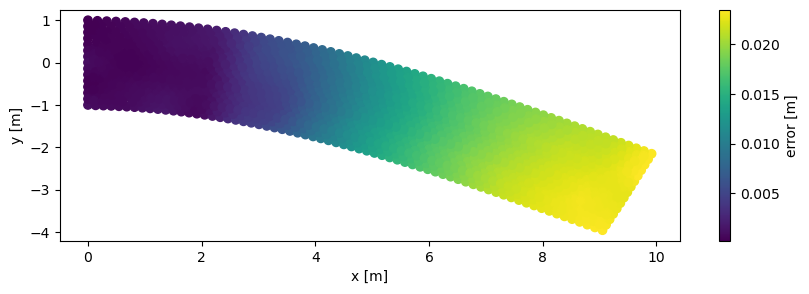
\includegraphics[width=0.8\textwidth]{Images/output_2D_beam.png}
    \end{figure}
\end{frame}

\begin{frame}
    \frametitle{Numerical Results - 3D Beam}
    In this case \( \Omega = [0, 10] \times [-1, 1] \times [-1, 1] \) with Dirichlet boundary conditions on \(\{0\} \times [-1, 1] \times [-1, 1]\) and a Neumann boundary condition on a random part of the remaining boundary.
    \vspace{0.5cm}

    The metric used to evaluate the performance of the method is the Root Mean Squared Error (RMSE) between the corrected solution and the fine solution.
    Here is a table with the results, testing the method on 100 different random simulations:
    \begin{table}
        \centering
        \begin{tabular}{|c|c|}
            \hline
            RMSE & 0.0257 ± 0.0274 m \\
            Extrema & 0.0004 \(\rightarrow\) 0.1370 m \\
            \hline
        \end{tabular}
    \end{table}
\end{frame}

\begin{frame}
    \frametitle{Numerical Results - 3D Beam}
    Here is an example of the corrected solution for a random simulation colored by the error:
    \begin{figure}
        \centering
        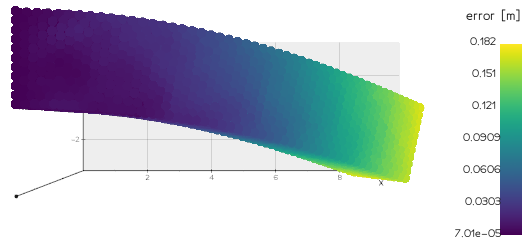
\includegraphics[width=0.8\textwidth]{Images/output_3D_beam.png}
    \end{figure}
\end{frame}

\begin{frame}
    \frametitle{Numerical Results: 2D Beam with BC}
    \begin{table}[h]
        \small
        \centering
        \begin{tabular}{|l|c|c|}
            \hline
            \textbf{Statistic} & \textbf{GNN} & \textbf{FC} \\ \hline
            RMSE Distribution (m) & 0.0059 ± 0.0072 & 0.0031 ± 0.0041 \\ \hline
            RMSE Extrema (m) & 0.0002 \(\rightarrow\) 0.0430 & 0.0001 \(\rightarrow\) 0.0382 \\ \hline
        \end{tabular}
        \caption{2D Beam Results}
    \end{table}
    \begin{figure}[h]
        \centering
        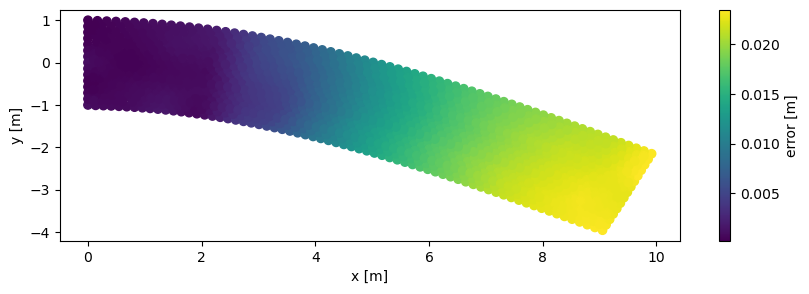
\includegraphics[width=0.6\textwidth]{Images/output_2D_beam.png}
        \caption{Placeholder for 2D Beam Results Image}
    \end{figure}
\end{frame}

\begin{frame}
    \frametitle{Numerical Results: 3D Beam with BC}
    \begin{table}[h]
        \small
        \centering
        \begin{tabular}{|l|c|c|}
            \hline
            \textbf{Statistic} & \textbf{GNN} & \textbf{FC} \\ \hline
            RMSE Distribution (m) & 0.0051 ± 0.0048 & 0.0055 ± 0.0048 \\ \hline
            RMSE Extrema (m) & 0.0002 \(\rightarrow\) 0.0351 & 0.0002 \(\rightarrow\) 0.0295 \\ \hline
        \end{tabular}
        \caption{3D Beam Results}
    \end{table}
    \begin{figure}[h]
        \centering
        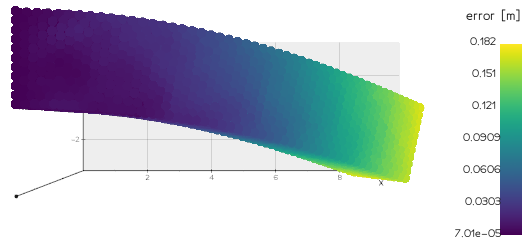
\includegraphics[width=0.6\textwidth]{Images/output_3D_beam.png}
        \caption{Placeholder for 3D Beam Results Image}
    \end{figure}
\end{frame}


\begin {frame}
    \frametitle{Comparison Summary BC vs No BC}
    \begin{table}[h]
        \small
        \centering
        \begin{tabular}{|l|c|c|}
            \hline
            \textbf{Model} & \textbf{RMSE (m) with BC} & \textbf{RMSE (m) without BC} \\ \hline
            2D Beam FC & 0.0031 ± 0.0041 & 0.0080 ± 0.0090 \\ \hline
            3D Beam FC & 0.0055 ± 0.0048 & 0.0257 ± 0.0274 \\ \hline
        \end{tabular}
        \caption{Comparison of RMSE between models with and without boundary conditions}
    \end{table}
\end{frame}

\begin{frame}
    \frametitle{Comparison with Existing Methods}
    \begin{table}[h]
        \small
        \centering
        \begin{tabular}{|l|c|c|}
            \hline
            \textbf{Method} & \textbf{MSE (m²)} & \textbf{MSE\textsubscript{max} (m²)} \\ \hline
            Our GNN 2D & 1.0e-4 ± 2.0e-4 & 0.0019 \\ \hline
            Our FC 2D & 1.0e-5 ± 1.0e-4 & 0.0015 \\ \hline
            DeepPhysics (a) & 5.4e-5 & 0.0370 \\ \hline
            DeepPhysics (b) & 6.6e-6 & 0.0050 \\ \hline
        \end{tabular}
        \caption{Comparison with DeepPhysics method}
    \end{table}
    
    \vspace{0.3cm}
    \small{
    \textbf{Note:} These results are not directly comparable as:
    \begin{itemize}
        \item Different length scales
        \item Different boundary conditions
        \item Different mesh resolutions
        \item Provided only as reference point for existing methods
    \end{itemize}
    }
\end{frame}



\iffalse
2D Beam:

GNN L2 ERROR Statistics :
        - Distribution : 0.162025 ± 0.197841 m
        - Extrema : 0.004288 -> 1.17872 m
        - Relative Distribution : 3.947784 ± 12.24652 %
        - Relative Extrema : 0.048002 -> 168.872635 %

GNN MSE Statistics :
        - Distribution : 8.7e-05 ± 0.000236 m²
        - Extrema : 0.0 -> 0.001853 m²
        - Relative Distribution : 0.551874 ± 5.994854 %
        - Relative Extrema : 8e-06 -> 95.059889 %

GNN RMSE Statistics :
        - Distribution : 0.005916 ± 0.007224 m
        - Extrema : 0.000157 -> 0.043041 m
        - Relative Distribution : 2.279254 ± 7.070532 %
        - Relative Extrema : 0.027714 -> 97.498661 %

FC L2 ERROR Statistics :
        - Distribution : 0.086031 ± 0.111081 m
        - Extrema : 0.003292 -> 1.047344 m
        - Relative Distribution : 2.406034 ± 8.429538 %
        - Relative Extrema : 0.054972 -> 0.899609 %

FC MSE Statistics :
        - Distribution : 2.6e-05 ± 0.000104 m²
        - Extrema : 0.0 -> 0.001463 m²
        - Relative Distribution : 0.256154 ± 2.173215 %
        - Relative Extrema : 1e-05 -> 0.269765 %

FC RMSE Statistics :
        - Distribution : 0.003141 ± 0.004056 m
        - Extrema : 0.00012 -> 0.038244 m
        - Relative Distribution : 1.389124 ± 4.866796 %
        - Relative Extrema : 0.031738 -> 0.51939 %

Comparison of RMSE between GNN and FC :
        - GNN : 0.005916 ± 0.007224 m
        - FC : 0.003141 ± 0.004056 m

\fi


\iffalse
3D Beam:

GNN L2 ERROR Statistics :
        - Distribution : 0.440302 ± 0.413019 m
        - Extrema : 0.017953 -> 3.043579 m
        - Relative Distribution : 7.173711 ± 17.297733 %
        - Relative Extrema : 0.162882 -> 207.40604 %

GNN MSE Statistics :
        - Distribution : 4.9e-05 ± 0.000106 m²
        - Extrema : 0.0 -> 0.001235 m²
        - Relative Distribution : 1.168912 ± 9.187474 %
        - Relative Extrema : 8.8e-05 -> 143.390884 %

GNN RMSE Statistics :
        - Distribution : 0.005084 ± 0.004769 m
        - Extrema : 0.000207 -> 0.035144 m
        - Relative Distribution : 4.141744 ± 9.986851 %
        - Relative Extrema : 0.09404 -> 119.745933 %

FC L2 ERROR Statistics :
        - Distribution : 0.473986 ± 0.41791 m
        - Extrema : 0.021292 -> 2.553303 m
        - Relative Distribution : 6.737772 ± 14.790396 %
        - Relative Extrema : 0.302738 -> 1.754084 %

FC MSE Statistics :
        - Distribution : 5.3e-05 ± 0.000105 m²
        - Extrema : 0.0 -> 0.000869 m²
        - Relative Distribution : 0.880511 ± 7.397949 %
        - Relative Extrema : 0.000306 -> 1.025603 %

FC RMSE Statistics :
        - Distribution : 0.005473 ± 0.004826 m
        - Extrema : 0.000246 -> 0.029483 m
        - Relative Distribution : 3.890054 ± 8.539239 %
        - Relative Extrema : 0.174786 -> 1.012721 %

Comparison of the RMSE between the GNN and the FC model:
        - GNN RMSE : 0.005084 ± 0.004769 m
        - FC RMSE : 0.005473 ± 0.004826 m
\fi

\iffalse
DeepPhysics results:
\begin{table}[h!]
    \centering
    \begin{tabular}{|l|c|c|c|}
        \hline
        \textbf{Name} & \textbf{MSE} & $\textbf{MSE}_{\text{max}}$ & $\textbf{SNR}^{dB}$ \\ \hline
        Beam (a) & $5.4 \times 10^{-5}$ & 0.0370 & 22.2 \\ \hline
        Beam (b) & $6.6 \times 10^{-6}$ & 0.0050 & 40.2 \\ \hline
    \end{tabular}
    \caption{Mean Squared Error (MSE), Maximum MSE, and Signal-to-Noise Ratio (SNR) for Beam and Propeller cases.}
    \label{tab:mse_snr}
\end{table}
\fi


\begin{frame}
    \frametitle{Strenghts of the Method}
    \textbf{Efficiency Without Compromise:}
    \begin{itemize}
        \item Starts with the coarse FEM solution, a robust approximation, and refines it using a neural network.
        \item Avoids solving a dense system of equations on fine meshes while ensuring the corrected solution retains physical fidelity.
    \end{itemize}
    \textbf{Topology Independence:}
    \begin{itemize}
        \item Adapts to various mesh topologies without requiring retraining.
        \item Interpolation of solutions onto a common grid ensures versatility across different geometries and mesh resolutions.
    \end{itemize}
\end{frame}

\begin{frame}
    \frametitle{Strenghts of the Method}
    \textbf{Interpretability:}
    \begin{itemize}
        \item Neural network corrections are grounded in a well-understood FEM baseline, avoiding the “black-box” behavior.
        \item Easier to diagnose and address errors, a critical factor for adoption in industrial and safety-critical contexts.
    \end{itemize}
    \textbf{Reduction of Error Accumulation in the Dynamic Case:}
    \begin{itemize}
        \item Predictions are tied to FEM output at each step, mitigating error propagation across time steps.
        \item Provides a clear advantage for applications requiring long temporal stability.
    \end{itemize}
\end{frame}

\begin{frame}
    \frametitle{Dynamic case}
    The final goal is to extend the method to the dynamic case. In that case some problems arise.
    \begin{itemize}
        \item Differences accumulate over time.
        \item The static model is not able to capture the dynamic behavior.
        \item How to capture data?
    \end{itemize}
    When the dynamic system behaves similarly to the static one, the static model works reasonably well.
\end{frame}

\begin{frame}
    \frametitle{Dynamic case - Ideas}
    Some ideas for the dynamic case:
    \begin{itemize}
        \item Create a new dataset containing both the solution and its time derivative, but keeping the same error as target.
        \item Creating two different datasets: one for the solution and one for the time derivative.
        \item Use a different network architecture capturing the time evolution. (But that would mean creating a black-box model).
    \end{itemize}
\end{frame}

\begin{frame}
    \frametitle{Conclusions}
    \begin{itemize}
        \item Introduced a hybrid method combining coarse FEM solutions with neural network corrections.
        \item Adapts to various mesh topologies without retraining.
        \item Provides interpretability by tying corrections to FEM outputs.
        \item Demonstrates potential for real-time applications.
    \end{itemize}
\end{frame}


\end{document}

\iffalse
TO COPILOT:


Based on your report, here’s a refined pitch that highlights the unique strengths of your method while addressing potential concerns about its perceived limitations:

---

**Title: A Hybrid Approach to Accelerating Finite Element Simulations Through Data-Driven Corrections**

**Introduction:**
Finite Element Modeling (FEM) remains a gold standard for solving complex PDEs in solid mechanics, but its high computational cost hinders its scalability for real-time and high-resolution simulations. This research introduces a novel hybrid approach combining FEM with neural networks to bridge this gap. Although currently demonstrated in static scenarios, the method lays the groundwork for significant advancements in simulation efficiency and adaptability.

---

**Key Innovations and Strengths of the Proposed Method:**

1. **Efficiency Without Compromise:**
   - Unlike pure neural network approaches that aim to predict full system dynamics (and suffer from instability and error accumulation), our method starts with the coarse FEM solution—a computationally cheap but robust approximation—and refines it using a neural network. 
   - This avoids solving a dense system of equations on fine meshes while ensuring the corrected solution retains physical fidelity.

2. **Topology Independence:**
   - By leveraging FEM's inherent flexibility, the approach adapts to various mesh topologies without requiring retraining, addressing a common limitation in many data-driven methods.
   - The interpolation of solutions onto a common grid ensures versatility across different geometries and mesh resolutions.

3. **Interpretability:**
   - Neural network corrections are grounded in a well-understood FEM baseline, avoiding the “black-box” behavior of methods like PINNs or MeshGraphNet. The method’s design makes it easier to diagnose and address errors, a critical factor for adoption in industrial and safety-critical contexts.

4. **Elimination of Error Accumulation:**
   - Unlike dynamic neural network approaches, which suffer from error propagation across time steps, our method mitigates this issue by anchoring predictions to FEM outputs at each step. This provides a clear advantage for applications requiring long temporal stability.

5. **Real-Time Potential:**
   - Once trained, the correction process involves a single forward pass through a neural network—a computationally lightweight operation. This significantly reduces simulation times while maintaining the desired accuracy, demonstrating promise for real-time and interactive applications.

---

**Broader Context and Future Prospects:**
While the immediate results are limited to static cases, the hybrid framework demonstrates clear scalability potential for dynamic simulations. Additionally, its modularity allows integration with advanced FEM solvers, contributing to the broader goal of enhancing simulation workflows rather than replacing existing methods outright.

This approach could pave the way for applications in:
- **Interactive Design:** Rapid prototyping and real-time deformation previews in CAD tools.
- **Medical Simulations:** Patient-specific modeling where computational resources are constrained.
- **Structural Analysis:** Scalable solutions for complex geometries in civil and aerospace engineering.

---

**Conclusion:**
This work presents a practical and interpretable solution to a long-standing challenge in computational mechanics. By combining the strengths of FEM with neural networks, it offers a middle ground between traditional and data-driven methods, demonstrating immediate value in static scenarios and long-term potential for broader adoption.

---

This pitch emphasizes the distinct advantages of your approach—interpretability, flexibility, and efficiency—making a compelling case for its current relevance and future impact. Let me know if you’d like further refinements!









That’s a valid concern, but let me clarify why the proposed method still holds an edge over PINNs in practical scenarios:

1. **Robustness vs. Direct Prediction:**
   - **Defense:** PINNs directly solve PDEs through optimization but are notoriously sensitive to hyperparameters, convergence issues, and problem complexity. In contrast, our method builds on the coarse FEM solution, which is a physically consistent and stable baseline. This makes it more robust and less prone to divergence, especially for challenging problems.

2. **Efficiency of Correction vs. Full Prediction:**
   - **Defense:** PINNs often require extensive training epochs to approximate solutions for a single problem setup. Our method uses the FEM solution as an intermediate step, effectively reducing the neural network’s learning burden to correcting localized errors. This results in faster and more reliable training.

3. **Interpretability and Debugging:**
   - **Defense:** A PINN’s black-box nature can make debugging difficult if the results deviate from expectations. Our method provides an interpretable pipeline where discrepancies can be traced back either to the FEM step or the correction network. This structured approach makes it more appealing for safety-critical or industrial applications.

4. **Dataset Cost vs. Training Cost:**
   - **Defense:** While it’s true that the dataset requires generating numerical simulations, this step only needs to be done once. The dataset can then generalize across similar problems or configurations, allowing rapid deployment of the trained correction model. PINNs, on the other hand, need to solve the optimization problem anew for every instance, making them computationally expensive in recurring simulations.

5. **Scalability to Complex Problems:**
   - **Defense:** For high-dimensional or highly irregular domains, PINNs face scalability issues due to the increasing complexity of loss terms (e.g., physics-based constraints). Our method offloads this complexity to the FEM solver, ensuring that the neural network only handles a simplified correction task. This division of labor ensures better scalability.

**Conclusion:**
Yes, our method involves some overhead in dataset preparation, but it more than compensates for this by offering improved robustness, interpretability, and scalability, especially for cases where multiple simulations share similar underlying physics or geometry. It’s a pragmatic middle-ground solution—leveraging the strengths of numerical methods and machine learning, rather than relying entirely on one or the other.

\fi

